\documentclass[a4paper]{article}

\usepackage{amsmath}
\usepackage{amssymb}
\usepackage{amsfonts}
\usepackage[style=iso]{datetime2}
\usepackage[explicit]{titlesec}
\usepackage{amsthm}
\usepackage{array}
\usepackage{graphicx}
\usepackage{float}
\usepackage[skip=1em,indent]{parskip}
\usepackage{caption}
\usepackage{hyperref}
\usepackage[sorting=none]{biblatex} %Imports biblatex package

\addbibresource{faulhabers_formula.bib} %Import the bibliography file

\graphicspath{ {./Images/} }

\theoremstyle{definition}
\newtheorem{problem}{Problem}
\newtheorem{definition}{Definition}

\begin{titlepage}
\title{Faulhaber's Formula and its Connection to Discrete Calculus}
\author{Abdul Musthakin}
\date{March 2025}
\end{titlepage}

\renewcommand{\thesection}{\Roman{section}}

\allowdisplaybreaks

\setlength{\parindent}{0pt}

\begin{document}
\maketitle

\section{Prerequisites}

You need very little to understand everything that will be discussed.
A decent number of new concepts will be introduced, but I plan on everything being self-contained.
The most important `prerequisite' is the ability to understand new things, and to follow the simple logic that will be used to go from one equation or formula to another.

Additionally, knowledge of basic calculus (derivatives, integrals, and the relationship between them) would certainly aid in one's appreciation for the results we will derive.
Whilst someone could technically understand everything without it, I do not think that there would be as much value in doing so.
Connections between that which is seemingly unrelated lies at the heart of what I deem to be interesting in mathematics -- which happens to be most things.
There is a very particular beauty in these connections.
The more you know beforehand, the more you have to link new concepts to.

Summation notation is required to be able to read, and by extension, understand, the maths presented here.
You could pick it up via the simple examples given in the introduction.
Regardless, prior experience is expected, and it is practically necessary to understand the way we will deal with sums in the later parts of the essay.

\section{Introduction}

The formula for the sum of the first $n$ positive integers is something that many people learn fairly early in school.
\begin{equation*}
    \sum_{i=1}^{n} i = 1 + 2 + 3 + \ldots + n = \frac{n(n+1)}{2}
\end{equation*}
The sum of the squares of the first $n$ positive integers, as well as the sum of the cubes, have reasonably well-known formulae as well.
\begin{align*}
    \sum_{i=1}^{n} i^2 & = \frac{n(n+1)(2n+1)}{6} \\
    \sum_{i=1}^{n} i^3 & = \frac{n^2 (n+1)^2}{4}
\end{align*}
These formulae are good and all, but how do we prove them?
We can take an algebraic approach, a geometric one, or we may simply use induction.
The latter method will always work as long as we already have an algebraic expression for the sum in terms of $n$.
What if we do not have the end result to prove?
Thus, the problem arises -- deriving a formula for the sum of the $k$-th powers of the first $n$ positive integers: Faulhaber's formula.
\begin{equation*}
    S_k(n) = \sum_{i=1}^{n} i^k = 1^k + 2^k + ... + n^k = \text{ ?}
\end{equation*}
$S_k$ is just another shorthand introduced; the previous three sums can be referred to as $S_1$, $S_2$, and $S_3$.
There are several ways of deriving Faulhaber's formula, and the method that I will use is not the most common one.
Whether or not it is the ``best" way cannot really be answered. To me, however, it is certainly the most interesting method.

\section{Necessary Definitions}

First, let us suppose that we have some sequence $a$, the $n$-th element of which is denoted by $a_n$.
Now, let us define the forward difference operator, $\Delta$, as follows.
\begin{equation}
    \Delta_n a_n = a_{n+1} - a_n
\end{equation}
Note that $\Delta$ applies to the sequence $a$, and not to $n$-th element of the sequence.
You could write $\Delta_n a_n$ as $(\Delta a)_n$, which may technically be more correct -- but it is more cumbersome to use.
This is just a minor detail.

The indefinite sum, or the antidifference, of a sequence can be defined in relation to the forward difference.
\begin{equation}
    \Delta_n \sum_n a_n = a_n
\end{equation}
That is, if $\sum_n a_n = A_n$, then
\begin{equation}
    A_{n+1} - A_n = a_n.
\end{equation}
Now, you may notice that this seems familiar.
Basic knowledge of calculus allows us to spot a connection.
We are dealing with differences and sums, but not in the way that found in regular calculus.
That is because this is not regular calculus.
Instead, we have ventured into the realm of the discrete, as opposed to the continuous which is much more familiar.

The forward difference is the discrete analogue to the derivative.
Whilst the latter measures the instantaneous rate of change of a function at some point, the former measures the rate of change of a sequence between two points.
Similarly, the antidifference is the discrete analogue to the antiderivative (indefinite integral).

Just as the fundamental theorem of calculus relates derivatives to integrals, we can construct a discrete version of it which relates forward differences to sums.
\begin{align}
    \Delta_n \sum_{i=n_0}^{n} a_i & = a_{n+1} \label{DFTC1}           \\
    \sum_{i=n_0}^n \Delta_i a_i   & = a_{n+1} - a_{n_0} \label{DFTC2}
\end{align}
The proof of these two statements is rather simple, only requiring the use of the definitions that we have already laid out, and the properties of sums.
The proof of the first statement is as follows.
\begin{align*}
    \Delta_n \sum_{i=n_0}^{n} a_i & = \sum_{i=n_0}^{n+1} a_i - \sum_{i=n_0}^{n} a_i         \\
                                  & = a_{n+1} + \sum_{i=n_0}^{n} a_i - \sum_{i=n_0}^{n} a_i \\
                                  & = a_{n+1} \quad \square
\end{align*}
The proof of the second statement does not require much more work than the first.
\begin{align*}
    \sum_{i=n_0}^n \Delta_i a_i & = \sum_{i=n_0}^n (a_{i+1} - a_i)                                \\
                                & = \sum_{i=n_0}^n a_{i+1} - \sum_{i=n_0}^n a_i                   \\
                                & = \sum_{i=n_0+1}^{n+1} a_i - \sum_{i=n_0}^n a_i                 \\
                                & = a_{n+1} - a_{n_0} + \sum_{i=n_0}^{n} a_i - \sum_{i=n_0}^n a_i \\
                                & = a_{n+1} - a_{n_0} \quad \square
\end{align*}
The relationship between the definite sum and its indefinite counterpart follows from the second statement.
\begin{equation}
    \sum_{i=n_0}^n a_n = \sum_{i=n_0}^n \Delta_n A_n = A_{n+1} - A_{n_0}
\end{equation}
Whilst we will not mention indefinite sums again, I thought that their inclusion here would serve to further illustrate the connection between regular old calculus, and what we have started to formulate.
More connections are to be found as we continue on.

There is just one more definition that needs to be made (kind of).
That is the falling factorial.
There are a few different notations for it, but the notation that I will be using is $x^{\underline{k}}$.
This may be read as ``$x$ to the falling $k$".
You can see the falling factorial as just the regular factorial, but with a specified end point.
\begin{equation}
    x^{\underline{k}} = x(x-1)(x-2)\cdots(x-k+1).
\end{equation}

\section{Formulating a Plan}

What we will do next makes a lot more sense if you see everything we have done so far as creating this discrete version of calculus.
The two most important concepts in calculus, the derivative and the integral, have already been translated over.
Consider the fact that you can find the derivative of any polynomial very easily with the power rule.
It would only make sense for there to be some discrete version of this -- a similar-looking rule to evaluate the forward difference of certain expressions.
Turns out there is, and it involves the falling factorial.
\begin{align*}
    \Delta_x x^{\underline{k}} & = (x+1)^{\underline{k}} - x^{\underline{k}}                     \\
                               & = (x+1)x(x-1)\cdots(x-k+2) - x(x-1)(x-2)\cdots(x-k+1)           \\
                               & = x(x-1)\cdots(x-k+2) \cdot [(x+1) - (x-k+1)]                   \\
                               & = kx(x-1)\cdots(x-k+2)                                          \\
                               & = kx^{\underline{k-1}} \stepcounter{equation}\tag{\theequation}
\end{align*}
Once again, we have an eerily familiar result.
Well, we best make use of it.

It is important to always be clear on what our goal is.
We have a sum to evaluate, and we have created some tools that resemble familiar concepts in calculus.
If instead of a sum, we had an integral to evaluate, one way of doing so would be to express the integrand (everything inside of the integral) as the derivative of something else.
Using the fact that derivatives and integrals are opposites of each other, we could then 'cancel them out' to get our answer.
This is the essence of the method that we will be using.

The sum of the falling factorial can be derived with what we have.
We simply have to rewrite it in terms of the forward difference of some expression, and then utilise \eqref{DFTC1}.
\begin{align*}
    \sum_{i=1}^n i^{\underline{k}} & = \sum_{i=1}^n \Delta_i \frac{i^{\underline{k+1}}}{k+1}                        \\
                                   & = \frac{(n+1)^{\underline{k+1}}}{k+1} - \frac{{1}^{\underline{k+1}}}{k+1}      \\
                                   & = \frac{(n+1)^{\underline{k+1}}}{k+1} \stepcounter{equation}\tag{\theequation}
\end{align*}
A result we used to simplify our expression above was that $x^{\underline{k}} = 0$ if $k > x$.
This is because $x-k+1$ will be less than or equal to 0 (thus one of the factors in the falling factorial will always be 0).
Since $k +1 > 1$ ($x^{\underline{k}}$ does not make sense otherwise), we were able to apply this.
Now, if we can express any sequence in terms of falling factorials, we can evaluate the sum of that sequence.

\section{Simple Cases}

Let us return to $S_1$, which we already have an expression for and can attempt to derive.
Via the definition of the falling factorial, $i^{\underline{1}}=i$.
Thus, formula for the sum of the first $n$ integers can be derived as follows.
\begin{align*}
    S_1 = \sum_{i=1}^{n} i & = \sum_{i=1}^{n} i^{\underline{1}} \\
                           & = \frac{(n+1)^{\underline{2}}}{2}  \\
                           & = \frac{n(n+1)}{2}
\end{align*}
It works!
Similarly, we can derive the formula for the sum of the squares of the first $n$ integers, $S_2$.
We need to find a way to express $i^2$ in terms of falling factorials first.
\begin{align*}
             & i^{\underline{2}} = i(i-1) = i^2 - i                                \\
    \leadsto & i^2 = i^{\underline{2}} + i = i^{\underline{2}} + i^{\underline{1}}
\end{align*}
The rest of the work simply involves using the ``reverse power rule" and simplifying the expression we get.
\begin{align*}
    S_2 & = \sum_{i=1}^{n} i^2                                                  \\
        & = \sum_{i=1}^{n} \left( i^{\underline{2}} + i^{\underline{1}} \right) \\
        & = \frac{(n+1)^{\underline{3}}}{3} + \frac{(n+1)^{\underline{2}}}{2}   \\
        & = \frac{n(n+1)(n-1)}{3} + \frac{n(n+1)}{2}                            \\
        & = \frac{2n(n+1)(n-1) + 3n(n+1)}{6}                                    \\
        & = \frac{n(n+1)[2(n-1) + 3]}{6}                                        \\
        & = \frac{n(n+1)(2n+1)}{6}
\end{align*}
The exact same process works for $S_3$.
\begin{align*}
             & i^{\underline{3}} = i(i-1)(i-2) = i^3 - 3i^2 + 2i                                                      \\
    \leadsto & i^3 = i^{\underline{3}} + 3i^2 - 2i = i^{\underline{3}} + 3i^{\underline{2}} + i^{\underline{1}}       \\
    \\
    S_3      & = \sum_{i=1}^n i^3                                                                                     \\                                                                                                     & = (i^{\underline{3}} + 3i^{\underline{2}} + i^{\underline{1}}) \\
             & = \frac{(n+1)^{\underline{4}}}{4} + 3\frac{(n+1)^{\underline{3}}}{3} + \frac{(n+1)^{\underline{2}}}{2} \\
             & = \frac{n(n+1)(n-1)(n-2)}{4} + n(n+1)(n-1) + \frac{n(n+1)}{2}                                          \\
             & = \frac{n(n+1)(n-1)(n-2)}{4} + \frac{4n(n+1)(n-1)}{4} + \frac{2n(n+1)}{4}                              \\
             & = \frac{n(n+1)(n-1)(n-2) + 4n(n+1)(n-1) +2n(n+1)}{4}                                                   \\
             & = \frac{n(n+1)[(n-1)(n-2) + 4(n-1) + 2]}{4}                                                            \\
             & = \frac{n(n+1)(n^2+n)}{4}                                                                              \\
             & = \frac{n^2(n+1)^2}{4}
\end{align*}

\section{Generalisation}

We now have a method to find $S_n$ for any $n$.
The amount of work required would increase with time, but the method itself does not change.
To generalise what we have done, first notice that expanding the falling factorial gives us a polynomial with certain coefficients.
\begin{align*}
    x^{\underline{1}} & = x                                     \\
    x^{\underline{2}} & = x^2 - x                               \\
    x^{\underline{3}} & = x^3 - 3x^2 + 2x                       \\
    x^{\underline{4}} & = x^{4} - 6 x^3 + 11 x^2 - 6 x          \\
    x^{\underline{5}} & = x^5 - 10 x^4 + 35 x^3 - 50 x^2 + 24 x \\
    \vdots
\end{align*}
When we rearrange these polynomials in order to get $x^k$ in terms of falling factorials, we get equations that resemble polynomials.
\begin{align*}
    x   & = x^{\underline{1}}                                                                                          \\
    x^2 & = x^{\underline{2}} + x^{\underline{1}}                                                                      \\
    x^3 & = x^{\underline{3}} + 3 x^{\underline{2}} + x^{\underline{1}}                                                \\
    x^4 & = x^{\underline{4}} + 6 x^{\underline{3}} + 7 x^{\underline{2}} + x^{\underline{1}}                          \\
    x^5 & = x^{\underline{5}} + 10 x^{\underline{4}} + 25 x^{\underline{3}} + 15 x^{\underline{2}} + x^{\underline{1}} \\
    \vdots
\end{align*}
This is the final thing we need.
We can evaluate $S_n$ simply by expanding and evaluating the sum of falling factorials.
There is just one problem: those coefficients.
They are called the Stirling numbers of the second kind, denoted as $S(k, i)$ or $k\brace i$, and they can be defined via the above expansion.
\begin{equation}
    x^k = \sum_{i=1}^k {k\brace i} x^{\underline{i}}
\end{equation}
For example,
\begin{equation*}
    x^5 = {5\brace 5} x^{\underline{5}} + {5\brace 4} x^{\underline{4}} + {5\brace 4} x^{\underline{3}} + {5\brace 3} x^{\underline{2}} + {5\brace 1} x^{\underline{1}}.
\end{equation*}
So far, that might feel a bit unsatisfying -- understandably so.
We had some coefficients we wanted to know more about (specifically how to calculate them in general), and we just gave them a name.
How does one actually go about calculating $k\brace i$?

Fortunately, we have recurrence formulae to work with.
Before we start deriving it, note that all $x^k$ can be expressed as the following.
\begin{equation*}
    x^k = \cdots + {k\brace k+2}x^{\underline{k+2}} + {k\brace k+1}x^{\underline{k+1}} + {k\brace k}x^{\underline{k}} + \cdots + {k\brace 1}x^{\underline{1}} + {k\brace 0}x^{\underline{0}}
\end{equation*}
I have just expanded out the definition above, whilst introducing a few extra terms.
This is just to show that this is valid to do, but any term with $k \brace i$, where $i > k$, equals zero.
Additionally, ${k \brace 0} = 0$ for all k, as can be seen by the absence of a $x^{\underline{0}}$ term in any of our above expansions.
${k\brace k} = 1$ for all k, and that is also fairly obvious from our above expansions.

With that out of the way, note the following.
\begin{equation*}
    x \cdot x^{\underline{k}} = x^{\underline{k}}(x-k) + kx^{\underline{k}} = x^{\underline{k+1}} + kx^{\underline{k}}
\end{equation*}
Using the definition of the Stirling numbers of the second kind, we have:
\begin{align*}
    x^{k+1} & =x\cdot x^k                                                                                         \\
            & = x \sum_{i=1}^{k} {k\brace i} x^{\underline{i}}                                                    \\
            & =\sum_{i=1}^{k} {k\brace i} x^{\underline{i+1}}+ \sum_{i=1}^{k} i{k\brace i} x^{\underline{i}}      \\
            & = \sum_{i=2}^{k+1} {k\brace i-1} x^{\underline{i}}+ \sum_{i=1}^{k} i{k\brace i} x^{\underline{i}}   \\
            & = \sum_{i=1}^{k+1} {k\brace i-1} x^{\underline{i}}+ \sum_{i=1}^{k+1} i{k\brace i} x^{\underline{i}} \\
            & = \sum_{i=1}^{k+1} \left({k\brace i-1} + i{k\brace i} \right)x^{\underline{i}}.
\end{align*}
We can express $x^{k+1}$ using a more direct approach.
\begin{equation*}
    x^{k+1} = \sum_{i=1}^{k+1} {{k+1}\brace {i}} x^{\underline{i}}
\end{equation*}
These two results can be equated to arrive at our recurrence formula.
\begin{align*}
    \sum_{i=1}^{k+1} {{k+1}\brace {i}} x^{\underline{i}} & = \sum_{i=1}^{k+1} \left({k\brace i-1} + i{k\brace i} \right)x^{\underline{i}} \\
    {{k+1}\brace {i}} x^{\underline{i}}                  & ={k\brace i-1} + i{k\brace i} \stepcounter{equation}\tag{\theequation}
\end{align*}
With this formula, and some initial values -- which we have -- we can find any Stirling number!
A possibly arduous process, sure, but certainly not more than working with increasingly long polynomials.

Now, we finally have everything we need.
Faulhaber's formula is ready to be presented in all its glory.
The sum of the $k$-th powers of the first $n$ positive integers can be written in terms of the Stirling numbers of the second kind and falling factorials.
\begin{align*}
    S_k & = \sum_{i=1}^n i^k                                                                              \\
        & = \sum_{i=1}^n \sum_{j=1}^k {k\brace j} i^{\underline{j}}                                       \\
        & = \sum_{j=1}^k {k\brace j} \sum_{i=1}^n i^{\underline{j}}      & \text{(Swapped order of sums)} \\
        & = \sum_{j=1}^k {k\brace j} \frac{(n+1)^{\underline{j+1}}}{j+1}
\end{align*}
With a swap of index variables, we get Faulhaber's formula.
\begin{equation}
    S_k = \sum_{i=1}^n i^k = \sum_{i=1}^k {k\brace i} \frac{(n+1)^{\underline{i+1}}}{i+1}
\end{equation}

\section{Conclusion and Additional Remarks}

Well, that is it.
We are done.
In the end, it only took a few lines to derive the formula which was our main goal the entire time.
The set-up was by far the lengthier portion, so perhaps that was time wasted.
Obviously, as I spent the time and effort required to write this, I do not believe that to be the case at all.

Faulhaber's formula is relatively simple.
It is not the most useful formula in the world, nor is it the prettiest.
However, putting everything aside, one can appreciate it for its simplicity.
Just a few concepts had to be introduced, and it ties them all in beautifully.
If the only benefit in doing this was to see that end result, then I would still consider it worth it.

The main value that was attained from this, I would argue, would be the connections that were made.
From what I have learnt about calculus in the past, I never would have expected it to link to something that is so `not continuous'.
Yet, discrete calculus is in a world of its own, and there is so much to the subject that cannot possibly be discussed in a brief essay such as this.

The Stirling numbers of the second kind have so much more to them as well.
Firstly they have a clear combinatorial interpretation.
$k\brace i$ is the number of ways to partition a set of $k$ elements into $i$ nonempty subsets.
The following diagram illustrates this well for the case where $k=4$.
\begin{figure}[H]
    \centering
    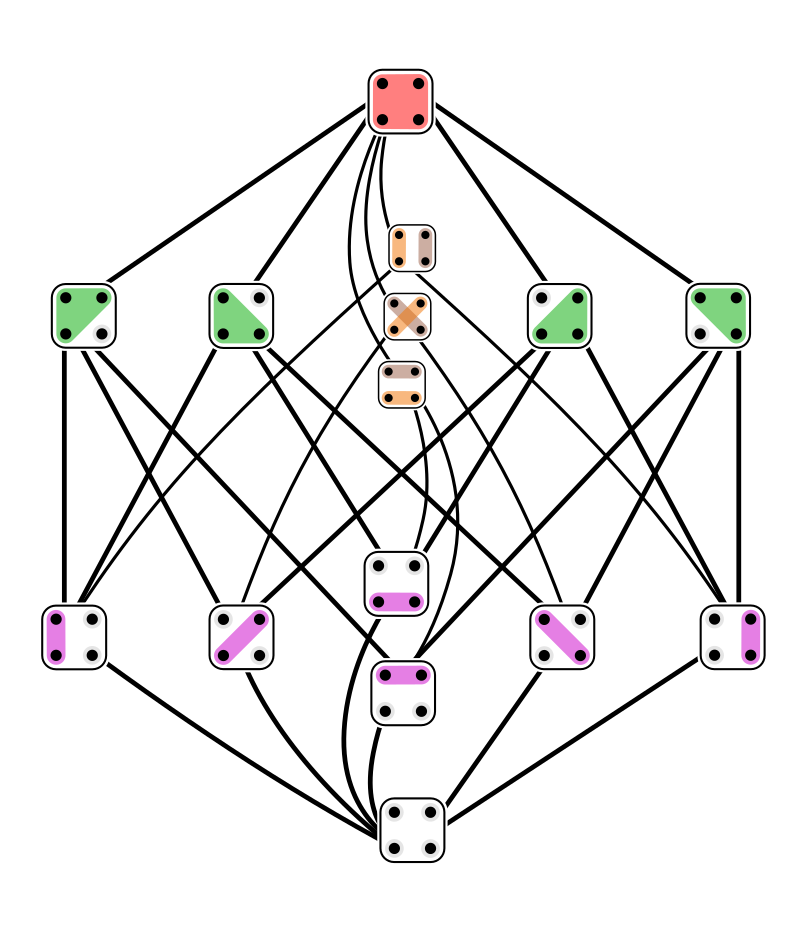
\includegraphics[width=8cm, keepaspectratio]{hasse_diagram.png}
    \captionsetup{justification=centering}
    \caption{Combinatorial Interpretation of S(4, i) Shown in a Hasse Diagram
        \\(Credits: Tilman Piesk, \href{https://creativecommons.org/licenses/by/3.0/}{CC BY 3.0}, via Wikimedia Commons)}
    \label{fig:fig1}
\end{figure}
Each colour is its own subset; uncoloured dots are within their own individual subsets.
$4\brace 1$ is on the top of the diagram and $4\brace 4$ is on the bottom.
Combinatorics can be used to show every result that we have shown via falling factorials \cite{MITSstirling}.

The previously cited article gives us a one-sum formula for the Stirling numbers of the second kind using the inclusion-exclusion principle.
\begin{equation*}
    {n\brace k} = \frac{1}{k!}\sum_{r=0}^{k}(-1)^r\binom{k}{r}(k-r)^n
\end{equation*}
Using the substitution $j = k - r$, we get:
\begin{align*}
    {n\brace k}  & = \frac{1}{k!}\sum_{j=0}^{k}(-1)^{k-j}\binom{k}{j}j^n                                      \\ \\
    {k \brace i} & = \frac{1}{i!} \sum_{j=0}^i (-1)^{i-j} \binom{i}{j} j^k & \text{(Swapping variable names)} \\
                 & = \frac{1}{i!} \sum_{j=1}^i (-1)^{i-j} \binom{i}{j} j^k                                    \\
                 & = \sum_{j=1}^i \frac{(-1)^{i-j}j^k}{(i-j)!j!}
\end{align*}
Faulhaber's formula may then be expressed explicitly as the following (just for fun).
\begin{equation*}
    \sum_{i=1}^n i^k = \sum_{i=1}^k \sum_{j=1}^i \frac{(-1)^{i-j}j^k (n+1)^{\underline{i+1}}}{(i+1)(i-j)!j!}
\end{equation*}

Moreover, Stirling numbers are related to probability and the Poisson distribution \cite{ADELL2019335}.
These connections are everywhere, and most of them you simply could not predict.
I find immense satisfaction in searching for these connections, and I hope that anyone reading this essay will share some of that satisfaction.
Deriving Faulhaber's formula was nice and all, but everything brought up along the way is where the true beauty lies.

\printbibliography

\end{document}